\section{Problem 3}
\label{part3}
\begin{verbatim}
Compute ratings for all the films that the substitute you have not seen.  Provide a list of
the top 5 recommendations for filmsthat the substitute you should see.  Provide a list of the bottom
5 recommendations (i.e., films the substitute you is almost certain to hate).
\end{verbatim}
\subsection{Solution}
\begin{enumerate}

\item Here I need to compute the ratings for the films my substitute has not seen. Now I need find out top 5 and bottom 5 recommendations for films that my substitute should see.
\item The bottom 5 recommendations are the films my substitute hate to see.
\item I have found these recommendations using a function called ``getRecommendations'' from recommendations.py.
\item The program for this question can be found in listing\ref{lst:q3-1}.
\item This function gives me a list of movies and their rating. These are recommendations for my substitute.
\item But all these are not considered as output, only the top 5 that is movies with rating as 5 are chosen and bottom 5 that is movies with rating  as 1 are chosen.
\item So these top 5 movies are recommended to my substitute expecting that he/she likes them.
\item The output file showing movie names and their ratings can be seen in fig\ref{Sample3t3}.

\newpage
\end{enumerate}
\subsection{Code Listing}

\lstinputlisting[language=Python,breaklines = true,frame=single,caption={Python Code for generating top 5 and least 5 movie recommendations that my substitute should see}, label=lst:q3-1,captionpos=b,numbers=left,showspaces=false,showstringspaces=false,basicstyle=\footnotesize]{mov_3.py}
\newpage

\subsection{Inputs}
\subsubsection{Sample u.data file}
\begin{figure}[ht]    
    \begin{center}
        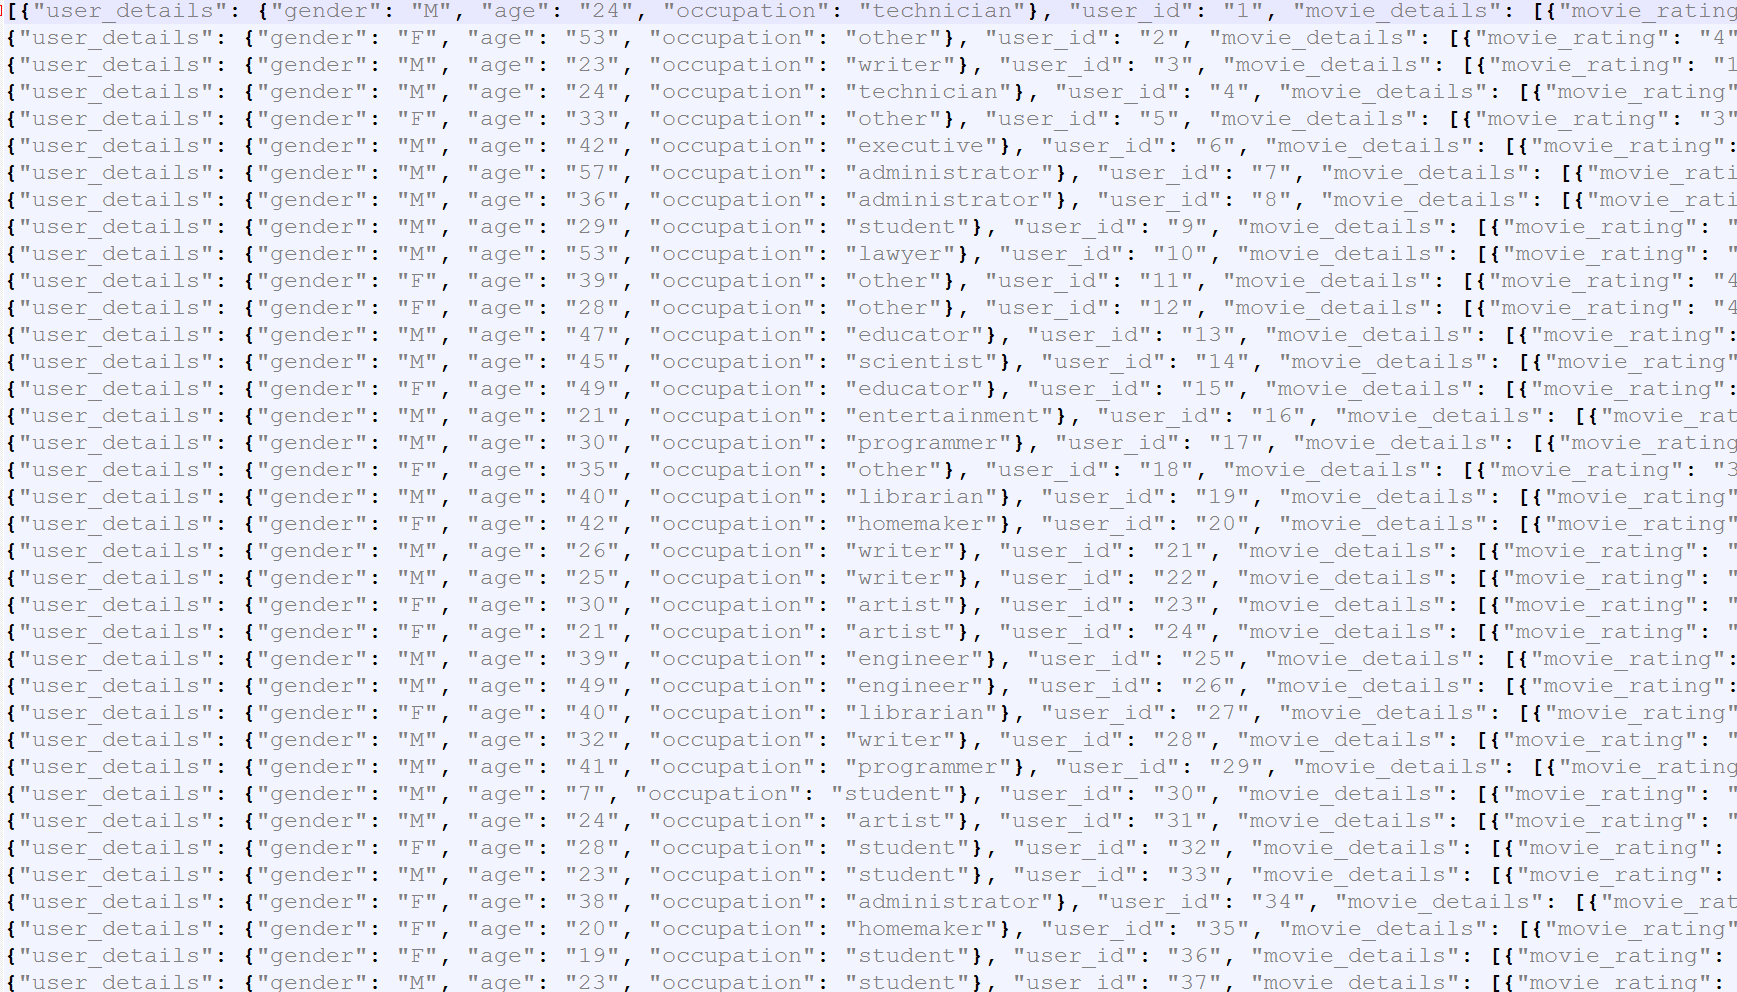
\includegraphics[scale=0.4]{sample_udata.png}
        \caption{Sample list of users and their rating for each movie}
        \label{Sample3t1}
    \end{center}
\end{figure}
\newpage
\subsubsection{Sample u.item file}
\begin{figure}[ht]    
    \begin{center}
        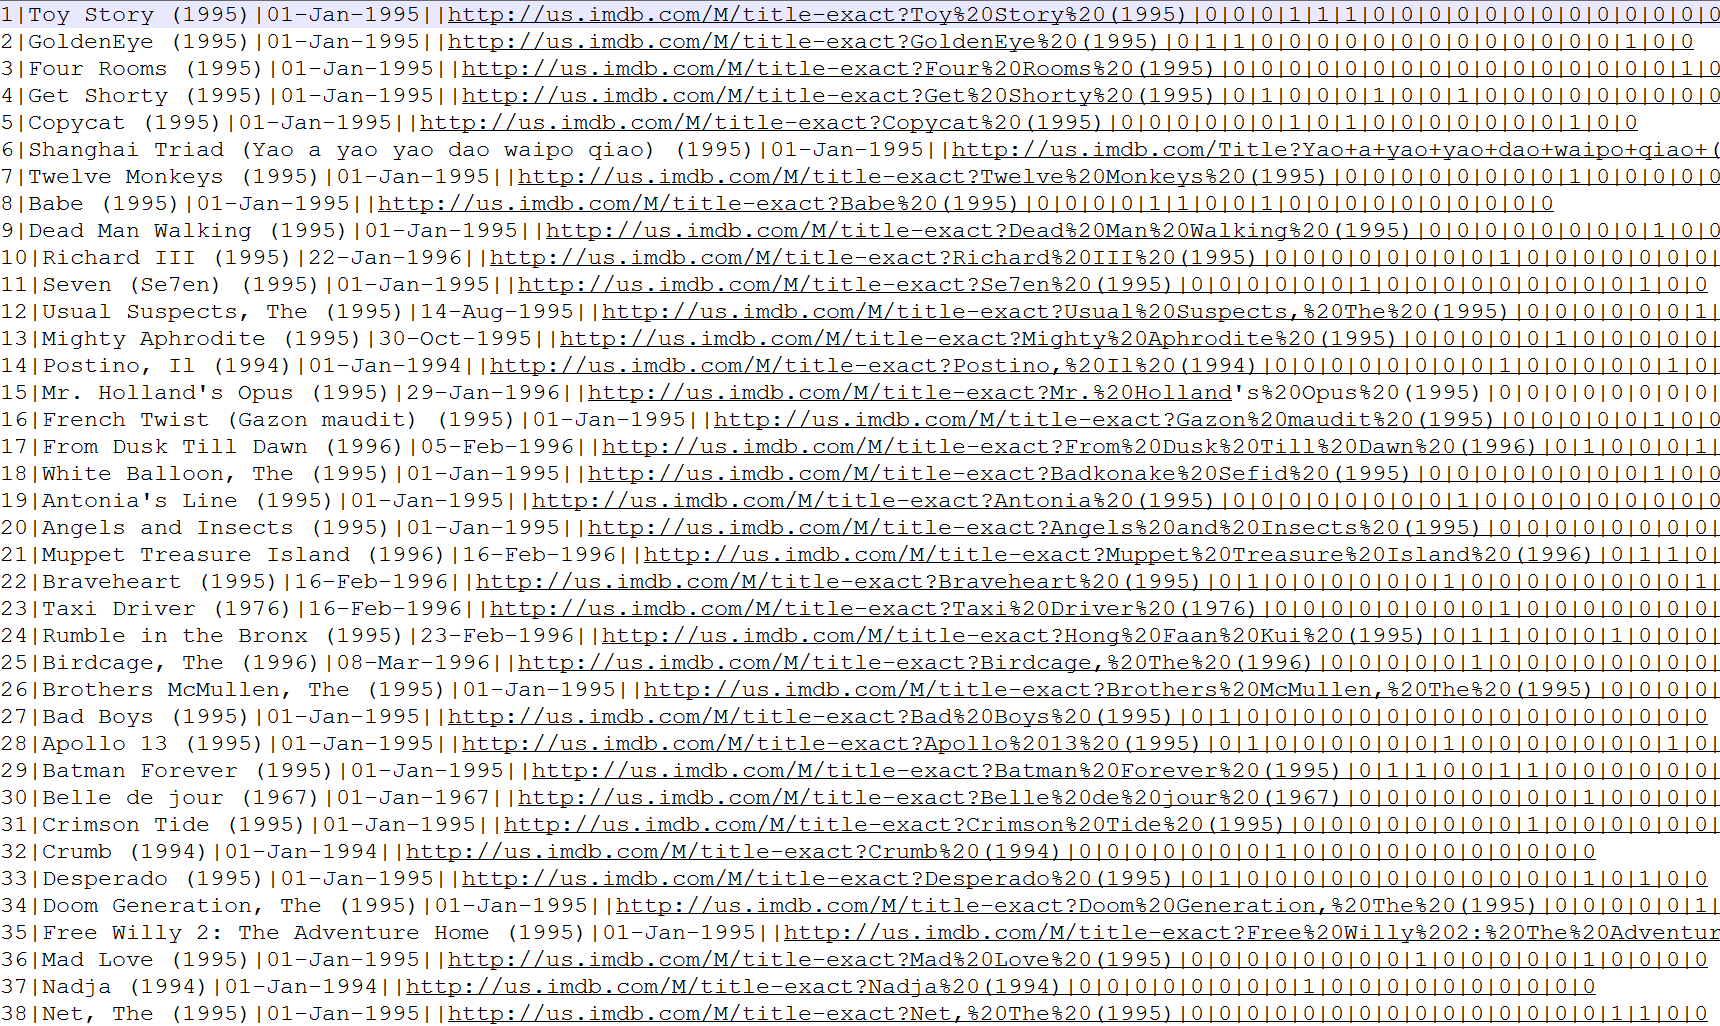
\includegraphics[scale=0.4]{sample_uitem.png}
        \caption{Sample list of movie data}
        \label{Sample3t2}
    \end{center}
\end{figure}
\newpage
\subsection{Outputs}
\subsubsection{Output file}
\begin{figure}[ht]    
    \begin{center}
        
\includegraphics[scale=0.8]{q3_output.png}
        \caption{File contains top 5 and least 5 movie recommendations that my substitute should see}
        \label{Sample3t3}
    \end{center}
\end{figure}
\newpage
